\documentclass{zc-ust-hw}

\usepackage{lipsum}
\usepackage{tikz-3dplot}

\newcommand*{\name}{SalahDin Rezk}
\newcommand*{\id}{202201079}
\newcommand*{\course}{MATH 201 - Linear Algebra and Vector Geometry}
\newcommand*{\assignment}{Assignment 1}

\begin{document}

\maketitle


%%%%%%%%%%%%%%%%%%%%
\section*{Question (1)}
%%%%%%%%%%%%%%%%%%%%

\begin{enumerate}
  \item Row reduce the matrix to echelon form. Identify the pivot positions in the final matrix and in the original matrix, and list the pivot columns.
    \begin{align*}
      \begin{bmatrix} 
        1 & 2 & 3 & 4 \\
        2 & 3 & 4 & 5 \\
        5 & 6 & 7 & 8
      \end{bmatrix} 
    \end{align*}

    \begin{align}
      2R_1-R_2\rightarrow R_2
          & \quad
          \begin{bmatrix} 
            \begin{array}{ccc|c}
              1 & 2 & 3 & 4 \\
              0 & 1 & 2 & 3 \\
              5 & 6 & 7 & 8
            \end{array}
          \end{bmatrix} \\
          -5R_1+R_3\rightarrow R_3
          & \quad
          \begin{bmatrix} 
            \begin{array}{ccc|c}
              1 & 2 & 3 & 4 \\
              0 & 1 & 2 & 3 \\
              0 & -4 & -8 & -12
            \end{array}
          \end{bmatrix} \\
          4R_2+R_3\rightarrow R_3
          & \quad
          \begin{bmatrix} 
            \begin{array}{ccc|c}
              1 & 2 & 3 & 4 \\
              0 & 1 & 2 & 3 \\
              0 & 0 & 0 & 0
            \end{array}
          \end{bmatrix}
        .\end{align}

        \begin{align}
          \text{Pivot positions: }
          \begin{bmatrix} 
            \begin{array}{ccc|c}
              \boxed{1} & 2 & 3 & 4 \\
              0 & \boxed{1} & 2 & 3 \\
              0 & 0 & 0 & 0
            \end{array}
          \end{bmatrix}
        .\end{align}

        \begin{align}
          \text{Pivot columns: }
          \begin{bmatrix} 
            \begin{array}{ccc|c}
              \smash{\color{black}\fbox{\color{black}\rule[-30pt]{0pt}{1pt}$1$}} & 2 & 3 & 4 \\
              0 & \smash{\color{black}\fbox{\color{black}\rule[-16.5pt]{0pt}{1pt}$1$}} & 2 & 3 \\
              0 & 0 & 0 & 0
            \end{array}
          \end{bmatrix}
        .\end{align}

      \item Suppose the system below is consistent for all possible values of $f$
        and $g$. What can you say about the coefficients $c$ and $d$? Justify your
        answer.
        \begin{align*}
          x_1+25x_2&=f \\
          cx_1+dx_2&=g
        .\end{align*}

        \begin{align}
          \begin{bmatrix} 
            \begin{array}{cc|c}
              1 & 25 & f \\
              c & d & g
            \end{array}
          \end{bmatrix}
        \end{align}
        \begin{align}
          R_2-cR_1\rightarrow R_2
          & \quad
          \begin{bmatrix} 
            \begin{array}{cc|c}
              1 & 25 & f \\
              0 & d-c25 & g-cf
            \end{array}
          \end{bmatrix}
        .\end{align}

        \begin{align}
          d-c25\neq 0
        .\end{align}

        If $d-c25=0$, then $g-cf=0$, which means that the system is inconsistent, since infinitely many values of $g$ and $f$ does not satisfy the equality. 
        \qed

      \item Apply the elementary row operations to reduce the augmented matrix
        of the following systems to the reduced row echelon form. Hence, find
        its solution, general solution form, or state that it has no solution
        whenever appropriate,
        \begin{enumerate}
          \item
            $\left[\begin{array}{llll}
                1 & 2 & 3 & 4 \\
                4 & 5 & 6 & 7 \\
                6 & 7 & 8 & 9
            \end{array}\right]$

            \begin{align}
              \frac{R_2-4R_1}{-3}\rightarrow R_2
              & \quad
              \begin{bmatrix} 
                \begin{array}{ccc|c}
                  1 & 2 & 3 & 4 \\
                  0 & 1 & 2 & 3 \\
                  6 & 7 & 8 & 9
                \end{array}
              \end{bmatrix} \\
              \frac{ R_3-6R_1 }{-5}\rightarrow R_3
              & \quad
              \begin{bmatrix} 
                \begin{array}{ccc|c}
                  1 & 2 & 3 & 4 \\
                  0 & 1 & 2 & 3 \\
                  0 & 1 & 2 & 3
                \end{array}
              \end{bmatrix} \\
              R_3-R_2\rightarrow R_3
              & \quad
              \begin{bmatrix} 
                \begin{array}{ccc|c}
                  1 & 2 & 3 & 4 \\
                  0 & 1 & 2 & 3 \\
                  0 & 0 & 0 & 0
                \end{array}
              \end{bmatrix}
            .\end{align}

            \begin{align}
              x+2y+3z&=4 \\
              y+2z&=3
            .\end{align}
            \begin{align}
              x&=4-2y-3z \\
              y&=3-2z
            .\end{align}
            \begin{align}
              x&=4-2(3-2z)-3z \\
               &=4-6+4z-3z \\
               &=z-2
             .\end{align}
             \begin{align}
               s.s.&=\left\{ \begin{bmatrix} z-2 \\ 3-2z \\ z \end{bmatrix} \right\} \\
                   &=\left\{ \begin{bmatrix} -2 \\ 3 \\ 0 \end{bmatrix}+z\begin{bmatrix} 1 \\ -2 \\ 1 \end{bmatrix} \right\}
                 .\end{align}

               \item 
                 $ \left[\begin{array}{llll}
                     1 & 3 & 5 & 7 \\
                     3 & 5 & 7 & 9 \\
                     5 & 7 & 9 & 1
                 \end{array}\right] $

                 \begin{align}
                   R_2-3R_1\rightarrow R_2
              & \quad
              \begin{bmatrix} 
                \begin{array}{ccc|c}
                  1 & 3 & 5 & 7 \\
                  0 & -4 & -8 & -12 \\
                  5 & 7 & 9 & 1
                \end{array}
              \end{bmatrix} \\
              R_3-5R_1\rightarrow R_3
              & \quad
              \begin{bmatrix} 
                \begin{array}{ccc|c}
                  1 & 3 & 5 & 7 \\
                  0 & -4 & -8 & -12 \\
                  0 & -8 & -16 & -34
                \end{array}
              \end{bmatrix} \\
              \frac{ R_3-2R_2 }{-4}\rightarrow R_3
              & \quad
              \begin{bmatrix} 
                \begin{array}{ccc|c}
                  1 & 3 & 5 & 7 \\
                  0 & -4 & -8 & -12 \\
                  0 & 0 & 0 & -5
                \end{array}
              \end{bmatrix}
            .\end{align}
            \begin{align}
              x+3y+5z&=7 \\
              -4y-8z&=-12 \\
              0&=-5
            .\end{align}
            \begin{align}
              s.s.&=\emptyset
            .\end{align}

        \end{enumerate}
    \end{enumerate}

    %%%%%%%%%%%%%%%%%%%%
    \section*{Question (2)}
    %%%%%%%%%%%%%%%%%%%%

    Determine if $b$ is a linear combination of the vectors formed from the
    columns of the matrix $A$.

    \begin{align*}
      A=\begin{bmatrix}1&-6&4\\0&6&7\\-3&18&-12\end{bmatrix}
      \quad
      b=\begin{bmatrix}2\\-7\\-2\end{bmatrix}
    \end{align*}

    \begin{gather}
      Ax=b\\
      \begin{bmatrix}1&-6&4\\0&6&7\\-3&18&-12\end{bmatrix}
      \begin{bmatrix}x\\y\\z\end{bmatrix}
      =\begin{bmatrix}2\\-7\\-2\end{bmatrix} \\
      \begin{bmatrix}x-6y+4z\\6y+7z\\-3x+18y-12z\end{bmatrix}
      =\begin{bmatrix}2\\-7\\-2\end{bmatrix}
    .\end{gather}

    \begin{align}
      \begin{bmatrix} 
        \begin{array}{ccc|c}
          1 & -6 & 4 & 2 \\
          0 & 6 & 7 & -7 \\
          -3 & 18 & -12 & -2
        \end{array}
      \end{bmatrix} 
    \end{align}
    \begin{align}
      R_3+3R_1\rightarrow R_3
      & \quad
      \begin{bmatrix} 
        \begin{array}{ccc|c}
          1 & -6 & 4 & 2 \\
          0 & 6 & 7 & -7 \\
          0 & 0 & 0 & -4
        \end{array}
      \end{bmatrix}
    .\end{align}

    \begin{align}
      x-6y+4z&=2 \\
      6y+7z&=-7 \\
      0&=-4
    .\end{align}
    \begin{align}
      s.s.&=\emptyset
    .\end{align}
    Vector $b$ is not a linear combination of the vectors formed from the columns
    of the matrix $A$. \qed

    %%%%%%%%%%%%%%%%%%%%
    \section*{Question (3)}
    %%%%%%%%%%%%%%%%%%%%

    \begin{enumerate}
      \item  Let ${v}_{{1}}=\left[\begin{array}{c}0 \\ 0 \\ -3\end{array}\right], {v}_{{2}}=\left[\begin{array}{c}0 \\ -6 \\ 6\end{array}\right]$, and ${v}_3=\left[\begin{array}{c}6 \\ -5 \\ 9\end{array}\right]$, does $\left\{{v}_1, {v}_2, {v}_3\right\}$ span $\mathbb{R}^3$? Why?

        \begin{align}
          \begin{bmatrix} 
            \begin{array}{ccc|c}
              0 & 0 & 6 & x \\
              0 & -6 & -5 & y \\
              -3 & 6 & 9 & z
            \end{array}
          \end{bmatrix}
        .\end{align}

        \begin{align}
          R_3 \leftrightarrow R_1
          & \quad
          \begin{bmatrix} 
            \begin{array}{ccc|c}
              -3 & 6 & 9 & z \\
              0 & -6 & -5 & y \\
              0 & 0 & 6 & x
            \end{array}
          \end{bmatrix} \\
          \frac{ R_1 }{-3}\rightarrow R_1
          & \quad
          \begin{bmatrix} 
            \begin{array}{ccc|c}
              1 & -2 & -3 & -z \\
              0 & -6 & -5 & y \\
              0 & 0 & 6 & x
            \end{array}
          \end{bmatrix} \\
          \frac{ R_2 }{-6}\rightarrow R_2
          & \quad
          \begin{bmatrix} 
            \begin{array}{ccc|c}
              1 & -2 & -3 & -z \\
              0 & 1 & \frac{5}{6} & -\frac{y}{6} \\
              0 & 0 & 6 & x
            \end{array}
          \end{bmatrix} \\
          R_1+2R_2\rightarrow R_1
          & \quad
          \begin{bmatrix} 
            \begin{array}{ccc|c}
              1 & 0 & -\frac{1}{3} & -\frac{z}{3} \\
              0 & 1 & \frac{5}{6} & -\frac{y}{6} \\
              0 & 0 & 6 & x
            \end{array}
          \end{bmatrix} \\
          \frac{ R_3 }{6}\rightarrow R_3
          & \quad
          \begin{bmatrix} 
            \begin{array}{ccc|c}
              1 & 0 & -\frac{1}{3} & -\frac{z}{3} \\
              0 & 1 & \frac{5}{6} & -\frac{y}{6} \\
              0 & 0 & 1 & \frac{x}{6}
            \end{array}
          \end{bmatrix} \\
          R_1+\frac{1}{3}R_3\rightarrow R_1
          & \quad
          \begin{bmatrix} 
            \begin{array}{ccc|c}
              1 & 0 & 0 & -\frac{z}{3}-\frac{x}{18} \\
              0 & 1 & \frac{5}{6} & -\frac{y}{6} \\
              0 & 0 & 1 & \frac{x}{6}
            \end{array}
          \end{bmatrix} \\
          R_2-\frac{5}{6}R_3\rightarrow R_2
          & \quad
          \begin{bmatrix} 
            \begin{array}{ccc|c}
              1 & 0 & 0 & -\frac{z}{3}-\frac{x}{18} \\
              0 & 1 & 0 & -\frac{y}{6}-\frac{5x}{36} \\
              0 & 0 & 1 & \frac{x}{6}
            \end{array}
          \end{bmatrix}
        .\end{align}

        $\left\{ v_1,v_2,v_3 \right\}$ spans $\mathbb{R}^3$ because the system of equations has a solution for all $x,y,z\in\mathbb{R}$. \qed

      \item For which value(s) of $h, k$ does $\left[\begin{array}{l}h \\
        k\end{array}\right]$ lie in
        $\operatorname{Span}\left\{\left[\begin{array}{c}2 \\
              -1\end{array}\right],\left[\begin{array}{l}2 \\
        1\end{array}\right]\right\}$ ?

        \begin{align}
          \begin{bmatrix} 
            \begin{array}{cc|c}
              2 & 2 & h \\
              -1 & 1 & k
            \end{array}
          \end{bmatrix}
        .\end{align}

        \begin{align}
          R_1+R_2\rightarrow R_1
        & \quad
        \begin{bmatrix} 
          \begin{array}{cc|c}
            1 & 3 & h+k \\
            -1 & 1 & k
          \end{array}
        \end{bmatrix} \\
        R_2+R_1\rightarrow R_2
        & \quad
        \begin{bmatrix} 
          \begin{array}{cc|c}
            1 & 3 & h+k \\
            0 & 4 & 2h+2k
          \end{array}
        \end{bmatrix} \\
        \frac{ R_2 }{4}\rightarrow R_2
        & \quad
        \begin{bmatrix} 
          \begin{array}{cc|c}
            1 & 3 & h+k \\
            0 & 1 & \frac{h+k}{2}
          \end{array}
        \end{bmatrix} \\
        R_1-3R_2\rightarrow R_1
        & \quad
        \begin{bmatrix} 
          \begin{array}{cc|c}
            1 & 0 & \frac{h-k}{2} \\
            0 & 1 & \frac{h+k}{2}
          \end{array}
        \end{bmatrix}
      .\end{align}

      \begin{align}
        s.s. = \mathbb{R}^2
      .\end{align}

      Since vectors $\begin{bmatrix} 2\\-1 \end{bmatrix} $ and $\begin{bmatrix} 2\\1 \end{bmatrix} $ spans $\mathbb{R}^2$, then any value for $h$ and $k$ lie in their span. \qed

    \item Let ${A}=\left[\begin{array}{ccc}2 & 0 & 6 \\ -1 & 8 & 5
      \\ 1 & -2 & 1\end{array}\right]$ and
      ${b}=\left[\begin{array}{c}10 \\ 3 \\ 3\end{array}\right]$.
      Denote the columns of ${A}$ by ${a}_1, {a}_2,
      {a}_3$ and let\\
      ${W}=\operatorname{Span}\left\{{a}_1, {a}_2, {a}_3\right\}$.

      \begin{enumerate}
        \item Is ${b}$ in $\left\{{a}_1, {a}_2, {a}_3\right\}$ ?

          Vector $b$ is not in the set $\left\{{a}_1, {a}_2, {a}_3\right\}$.

        \item Is ${b}$ in ${W}$ ?

          \begin{align}
            \begin{bmatrix} 
              \begin{array}{ccc|c}
                2 & 0 & 6 & 10 \\
                -1 & 8 & 5 & 3 \\
                1 & -2 & 1 & 3
              \end{array}
            \end{bmatrix}
          .\end{align}
          \begin{align}
            R_1\leftrightarrow R_3
            & \quad
            \begin{bmatrix} 
              \begin{array}{ccc|c}
                1 & -2 & 1 & 3 \\
                -1 & 8 & 5 & 3 \\
                2 & 0 & 6 & 10
              \end{array}
            \end{bmatrix} \\
            R_2+R_1\rightarrow R_2
            & \quad
            \begin{bmatrix} 
              \begin{array}{ccc|c}
                1 & -2 & 1 & 3 \\
                0 & 6 & 6 & 6 \\
                2 & 0 & 6 & 10
              \end{array}
            \end{bmatrix} \\
            R_3-2R_1\rightarrow R_3
            & \quad
            \begin{bmatrix} 
              \begin{array}{ccc|c}
                1 & -2 & 1 & 3 \\
                0 & 6 & 6 & 6 \\
                0 & 4 & 4 & 4
              \end{array}
            \end{bmatrix} \\
            R_2\leftrightarrow R_3
            & \quad
            \begin{bmatrix} 
              \begin{array}{ccc|c}
                1 & -2 & 1 & 3 \\
                0 & 4 & 4 & 4 \\
                0 & 6 & 6 & 6
              \end{array}
            \end{bmatrix} \\
            R_3-\frac{3}{2}R_2\rightarrow R_3
            & \quad
            \begin{bmatrix} 
              \begin{array}{ccc|c}
                1 & -2 & 1 & 3 \\
                0 & 4 & 4 & 4 \\
                0 & 0 & 0 & 0
              \end{array}
            \end{bmatrix}
          .\end{align}
          Since the system is consistent, then $b$ is in $W$. \qed

      \end{enumerate}

  \end{enumerate}

\section*{Question (4)}

Describe the solutions of the first system of equations below in parametric
vector form. Provide a geometric comparison with the solution set of the second
system of equations below. 

\begin{equation*}\begin{array}{rlrl}
  4 x_1+4 x_2+8 x_3 & =16 & \quad 4 x_1+4 x_2+8 x_3 & =0 \\
  -12 x_1-12 x_2-24 x_3 & =-48 & \quad -12 x_1-12 x_2-24 x_3 & = 0 \\
  -7 x_2-21 x_3 & =14 & \quad -7 x_2-21 x_3 & = 0
\end{array}\end{equation*}

\begin{align}
  \begin{bmatrix} 
    \begin{array}{ccc|c}
      4 & 4 & 8 & 16 \\
      -12 & -12 & -24 & -48 \\
      0 & -7 & -21 & 14
    \end{array}
  \end{bmatrix}
.\end{align}
\begin{align}
  \frac{R_1}{4}\rightarrow R_1
  & \quad
  \begin{bmatrix} 
    \begin{array}{ccc|c}
      1 & 1 & 2 & 4 \\
      -12 & -12 & -24 & -48 \\
      0 & -7 & -21 & 14
    \end{array}
  \end{bmatrix} \\
  R_2+12R_1\rightarrow R_2
  & \quad
  \begin{bmatrix} 
    \begin{array}{ccc|c}
      1 & 1 & 2 & 4 \\
      0 & 0 & 0 & 0 \\
      0 & -7 & -21 & 14
    \end{array}
  \end{bmatrix} \\
  R_2 \leftrightarrow R_3
  & \quad
  \begin{bmatrix} 
    \begin{array}{ccc|c}
      1 & 1 & 2 & 4 \\
      0 & -7 & -21 & 14 \\
      0 & 0 & 0 & 0
    \end{array}
  \end{bmatrix} \\
  \frac{R_2}{-7}\rightarrow R_2
  & \quad
  \begin{bmatrix} 
    \begin{array}{ccc|c}
      1 & 1 & 2 & 4 \\
      0 & 1 & 3 & -2 \\
      0 & 0 & 0 & 0
    \end{array}
  \end{bmatrix}
.\end{align}

\begin{align}
  x + y + 2z &= 4 \\
  y + 3z &= -2
\end{align}
\begin{align}
  x &= 4 - y - 2z \\
  y &= -2 - 3z
.\end{align}
\begin{align}
  x &= 4 - (-2 - 3z) - 2z \\
  x &= 4 + 2 + 3z - 2z \\
  x &= 6 + z
.\end{align}

\begin{align}
  {s.s.}_1 &= \left\{ \begin{bmatrix} 6 \\ -2 \\ 0 \end{bmatrix} + z \begin{bmatrix} 1 \\ -3 \\ 1 \end{bmatrix} \right\} \\
  {s.s}_2 &= \left\{ z \begin{bmatrix} 1 \\ -3 \\ 1 \end{bmatrix} \right\} 
.\end{align}

\begin{figure}[htpb]
  \centering
  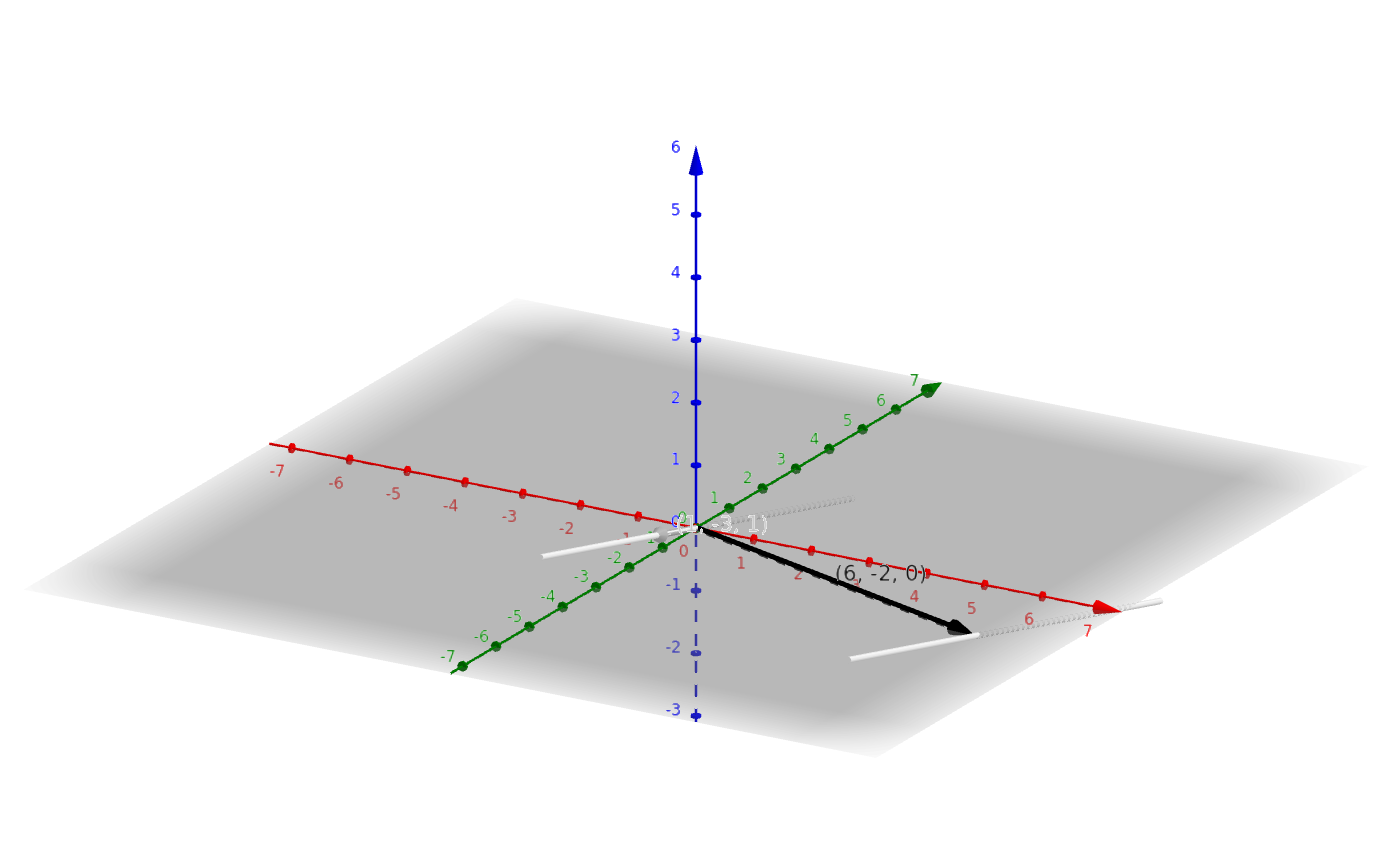
\includegraphics[width=0.8\textwidth]{vectors.png}
  \caption{Vector equations results in two parallel lines as there is only one degree of freedom.}
  \label{fig:vectors-png}
\end{figure}

\end{document}
